\documentclass[14pt,aspectratio=169]{beamer}
\usepackage{ifxetex}
\ifxetex
  \usepackage{fontspec}
\else
  \usepackage[T1]{fontenc}
  \usepackage[utf8]{inputenc}
\fi
\usepackage{pifont}% http://ctan.org/pkg/pifont
\newcommand{\cmark}{\ding{51}}%
%\newcommand{\xmark}{\ding{55}}%

\usepackage[english]{babel}
\uselanguage{english}
\usetheme{simple}
\usecolortheme{whiteonblack}
\usepackage{array}
\usepackage{aurl}
\daurl{meta}{http://www.snik.eu/ontology/meta/}
\daurl{ob}{http://www.snik.eu/ontology/ob/}
\daurl{bb}{http://www.snik.eu/ontology/bb/}
\usepackage{url}
\usepackage{graphicx}
\usepackage{csquotes}
\usepackage{amssymb}
\usepackage{pifont}
\newcommand{\xmark}{\ding{55}}%
\newcolumntype{H}{>{\setbox0=\hbox\bgroup}c<{\egroup}@{}} % comment out columns
\date{2024-09-17}
\author{\texorpdfstring{Konrad Höffner\newline{}Institut für Medizinische Informatik, Statistik und Epidemiologie (IMISE)\newline{}\url{konrad.hoeffner@uni-leipzig.de}}{Konrad Höffner}}
\title{RickView: Robuster, leichtgewichtiger, unabhängiger und performanter Wissensgraphen-Browser}
\subtitle{}

\newcommand{\imageslide}[4][]
{
\begin{frame}[plain]{~~~~#2}
\vspace{0.2em}
\centering\makebox[\linewidth]{\includegraphics[width=1.13\linewidth,height=0.88\textheight,keepaspectratio]{#3}}
\\#1
\note{#4}
\end{frame}
}

\begin{document}

%\begin{frame}
%\titlepage
%\end{frame}

\begin{frame}[plain]
\centering\makebox[\linewidth]{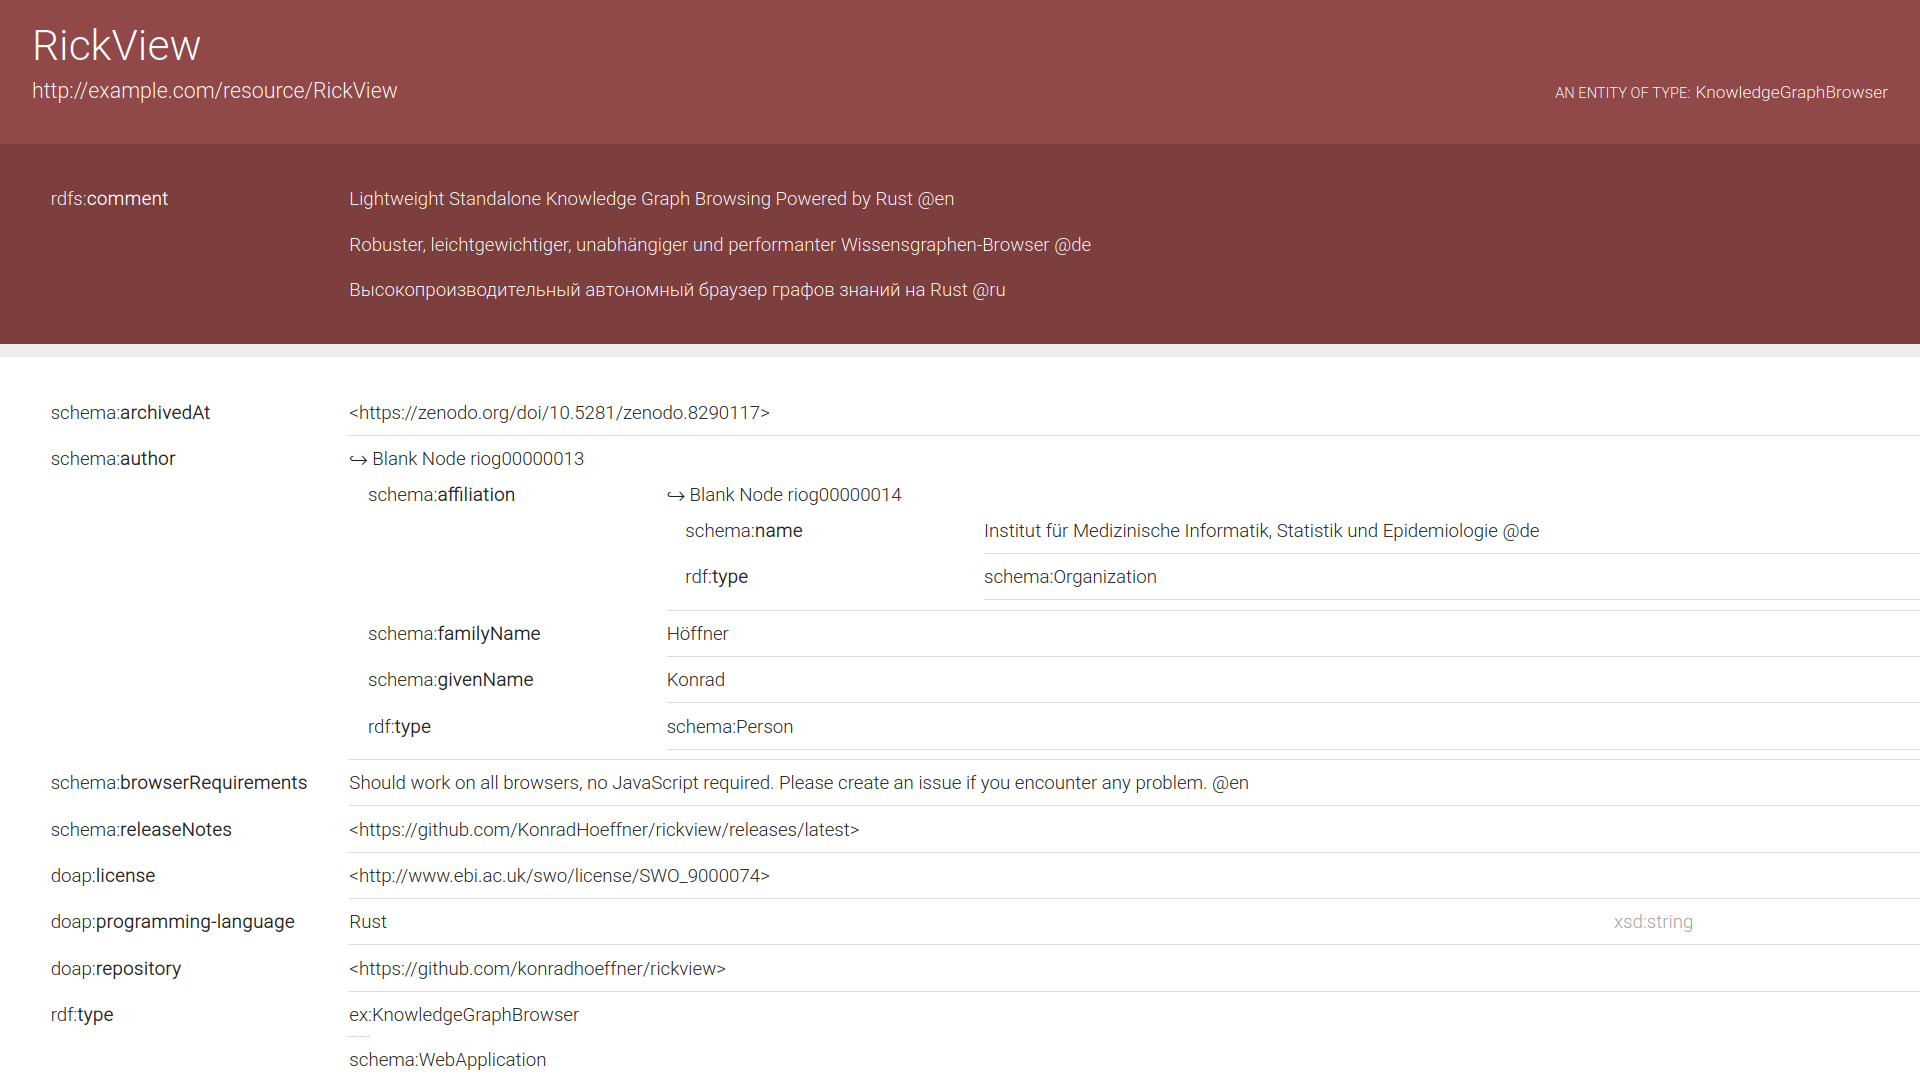
\includegraphics[width=1.13\linewidth,height=\textheight,keepaspectratio]{img/rickview-self.png}}
\end{frame}

\imageslide[aufwändige Einrichtung\\hoher Ressourcenaufwand\\fehleranfällig]{SPARQL-zentrierte Architektur}{img/architecture.pdf}{}
\imageslide[\url{https://github.com/KonradHoeffner/rickview}]{Architektur von RickView}{img/architecture-simple.pdf}{}
%\imageslide{Simplified Architecture}{img/architecture-simple.pdf}{}
%\imageslide{RickView Architecture}{img/architecture-rickview.pdf}{}

\end{document}
